%-------------------------------------------------------------------------------
\begin{frame}
\createtitle{Methods}
\pause
\begin{itemize}
\item 4 VTs (\texttt{ViT} \tinycite{dosovitskiy2020image}, \texttt{Swin} \tinycite{liu2021swin}, \texttt{DeiT} \tinycite{touvron2021training}, and \texttt{BeiT} \tinycite{bao2022beit}) versus 4 CNNs (\texttt{ResNet} \tinycite{he2016deep}, \texttt{VGG} \tinycite{simonyan2014very}, \texttt{ConvNext} \tinycite{liu2022convnet}, and \texttt{EfficientNetV2} \tinycite{tan2021efficientnetv2});
\begin{itemize}
\item All pre-trained on ImageNet1K;
\end{itemize}
\pause
\item Off-the-shelf and fine-tuning experiments on ...
\pause
\item ... those 3 tasks from the ``\textit{Rijksmuseum Challenge}'';
\begin{itemize}
\pause
\item Problems:
\begin{itemize}
\item Big (112K images);
\item Many classes;
\item Unbalanced;
\end{itemize}
\pause
\item Solutions:
\begin{itemize}
\item Taking top 30 classes;
\item Max of 1K images per class;
\end{itemize}
\pause
\item Bonus:
\begin{itemize}
\item Dataset sizes now between 6.5K and 9K;
\item Randomly generating 5 subsets per task for extra robustness.
\end{itemize}
\end{itemize}
\end{itemize}
\end{frame}
%-------------------------------------------------------------------------------

%-------------------------------------------------------------------------------
\begin{frame}
\createtitle{Off the shelf results}
\centering
{\tiny \textbf{Validation accuracy during training}}
\def\svgwidth{\textwidth}
\input{img/ots_mean_accuracy.pdf_tex}

\vspace{0.3cm}

\resizebox{\columnwidth}{!}{%
\begin{tabular}{lllllll}
\hline
\textbf{Model} & \textbf{Type} &  & \textbf{Material} & & \textbf{Artist} & \\
& \textbf{Accuracy} & \textbf{Bal. accuracy} & \textbf{Accuracy} & \textbf{Bal. accuracy} & \textbf{Accuracy} & \textbf{Bal. accuracy} \\ \hline
\textbf{vit\_b\_16} & 86.06\% $_{\pm 1.06\%}$ & 84.13\% $_{\pm 1.57\%}$ & 81.78\% $_{\pm 0.48\%}$ & 67.38\% $_{\pm 1.37\%}$ & 84.89\% $_{\pm 0.46\%}$ & 81.42\% $_{\pm 0.42\%}$  \\
\textbf{swin\_b} & \cellcolor{bestcol}89.43\% $_{\pm 0.93\%}$ & \cellcolor{bestcol}87.47\% $_{\pm 1.02\%}$ & \cellcolor{bestcol}85.87\% $_{\pm 0.35\%}$ & \cellcolor{bestcol}71.19\% $_{\pm 1.60\%}$ & \cellcolor{bestcol}90.40\% $_{\pm 0.65\%}$ & \cellcolor{bestcol}88.64\% $_{\pm 0.78\%}$  \\
\textbf{beit\_b\_16} & \cellcolor{worstcol}82.26\% $_{\pm 0.72\%}$ & \cellcolor{worstcol}77.75\% $_{\pm 0.27\%}$ & 76.87\% $_{\pm 0.96\%}$ & 60.16\% $_{\pm 1.56\%}$ & 79.70\% $_{\pm 0.69\%}$ & 75.35\% $_{\pm 1.09\%}$  \\
\textbf{deit\_b\_16} & 88.18\% $_{\pm 0.66\%}$ & 85.36\% $_{\pm 0.54\%}$ & 82.80\% $_{\pm 1.12\%}$ & 66.46\% $_{\pm 1.03\%}$ & 88.13\% $_{\pm 0.76\%}$ & 85.62\% $_{\pm 0.87\%}$  \\\hdashline
\textbf{vgg19} & 83.93\% $_{\pm 0.72\%}$ & 83.35\% $_{\pm 0.81\%}$ & 76.87\% $_{\pm 0.44\%}$ & 61.39\% $_{\pm 1.47\%}$ & 82.01\% $_{\pm 0.66\%}$ & 78.10\% $_{\pm 0.77\%}$  \\
\textbf{resnet50} & 85.51\% $_{\pm 0.64\%}$ & 82.33\% $_{\pm 1.85\%}$ & 80.99\% $_{\pm 0.82\%}$ & 65.51\% $_{\pm 0.93\%}$ & 87.71\% $_{\pm 1.06\%}$ & 85.12\% $_{\pm 1.34\%}$  \\
\textbf{eff. netv2\_m} & 83.41\% $_{\pm 0.76\%}$ & 82.05\% $_{\pm 1.25\%}$  & \cellcolor{worstcol}75.96\% $_{\pm 1.24\%}$ & \cellcolor{worstcol}59.15\% $_{\pm 1.24\%}$ & \cellcolor{worstcol}78.62\% $_{\pm 1.07\%}$ & \cellcolor{worstcol}73.92\% $_{\pm 0.96\%}$  \\
\textbf{convnext\_b} & \cellcolor{secondbestcol}89.19\% $_{\pm 0.64\%}$ & \cellcolor{secondbestcol}86.95\% $_{\pm 1.38\%}$ & \cellcolor{secondbestcol}84.14\% $_{\pm 0.92\%}$ & \cellcolor{secondbestcol}69.10\% $_{\pm 1.05\%}$ & \cellcolor{secondbestcol}90.13\% $_{\pm 0.94\%}$ & \cellcolor{secondbestcol}87.84\% $_{\pm 1.07\%}$  \\\hline
\end{tabular}
}
\centering
{\tiny \textbf{Testing performance}}

\end{frame}
%-------------------------------------------------------------------------------

%-------------------------------------------------------------------------------
\begin{frame}
\createtitle{Fine-tuning results}
\centering
{\tiny \textbf{Validation accuracy during training}}
\def\svgwidth{\textwidth}
\input{img/ft_mean_accuracy.pdf_tex}

\vspace{0.3cm}

\resizebox{\columnwidth}{!}{%
\begin{tabular}{lllllll}
\hline
\textbf{Model} & \textbf{Type} &  & \textbf{Material} & & \textbf{Artist} & \\
& \textbf{Accuracy} & \textbf{Bal. accuracy} & \textbf{Accuracy} & \textbf{Bal. accuracy} & \textbf{Accuracy} & \textbf{Bal. accuracy} \\ \hline
\textbf{vit\_b\_16} & \cellcolor{worstcol}90.11\% $_{\pm 0.35\%}$ & 87.40\% $_{\pm 0.29\%}$ & 87.42\% $_{\pm 0.45\%}$ & 73.46\% $_{\pm 1.44\%}$ & 92.05\% $_{\pm 0.44\%}$ & 89.77\% $_{\pm 0.38\%}$  \\
\textbf{swin\_b} & \cellcolor{bestcol}92.17\% $_{\pm 0.98\%}$ & \cellcolor{secondbestcol}89.71\% $_{\pm 1.03\%}$ & \cellcolor{bestcol}89.35\% $_{\pm 0.68\%}$ & 77.16\% $_{\pm 2.98\%}$ & \cellcolor{bestcol}95.05\% $_{\pm 0.47\%}$ & \cellcolor{bestcol}93.94\% $_{\pm 0.81\%}$  \\
\textbf{beit\_b\_16} & 90.81\% $_{\pm 0.41\%}$ & 87.95\% $_{\pm 0.69\%}$ & \cellcolor{worstcol}85.74\% $_{\pm 0.37\%}$ & \cellcolor{worstcol}72.12\% $_{\pm 1.38\%}$ & \cellcolor{worstcol}91.27\% $_{\pm 1.13\%}$ & \cellcolor{worstcol}88.83\% $_{\pm 1.63\%}$  \\
\textbf{deit\_b\_16} & 91.78\% $_{\pm 0.64\%}$ & 89.22\% $_{\pm 0.90\%}$ & 87.85\% $_{\pm 1.12\%}$ & 74.42\% $_{\pm 1.99\%}$ & 93.37\% $_{\pm 1.15\%}$ & 91.67\% $_{\pm 1.55\%}$  \\\hdashline
\textbf{vgg19} & 90.54\% $_{\pm 0.37\%}$ & \cellcolor{worstcol}87.05\% $_{\pm 1.03\%}$ & 85.74\% $_{\pm 1.40\%}$ & 72.43\% $_{\pm 3.03\%}$ & 92.20\% $_{\pm 0.49\%}$ & 90.18\% $_{\pm 0.72\%}$  \\
\textbf{resnet50} & 91.78\% $_{\pm 0.44\%}$ & 88.24\% $_{\pm 0.59\%}$ & 88.69\% $_{\pm 0.99\%}$ & \cellcolor{secondbestcol}77.97\% $_{\pm 2.25\%}$ & \cellcolor{secondbestcol}94.72\% $_{\pm 0.74\%}$ & \cellcolor{secondbestcol}93.41\% $_{\pm 1.05\%}$  \\
\textbf{eff. netv2\_m} & 90.87\% $_{\pm 0.67\%}$ & 88.34\% $_{\pm 1.37\%}$ & 87.55\% $_{\pm 1.15\%}$ & 75.31\% $_{\pm 1.60\%}$ & 92.65\% $_{\pm 0.54\%}$ & 90.84\% $_{\pm 0.51\%}$  \\
\textbf{convnext\_b} & \cellcolor{secondbestcol}92.15\% $_{\pm 0.40\%}$ & \cellcolor{bestcol}89.82\% $_{\pm 1.18\%}$ & \cellcolor{secondbestcol}88.79\% $_{\pm 1.07\%}$ & \cellcolor{bestcol}78.40\% $_{\pm 1.26\%}$ & 94.60\% $_{\pm 0.54\%}$ & 93.13\% $_{\pm 0.61\%}$  \\\hline
\end{tabular}
}
\centering
{\tiny \textbf{Testing performance}}

\end{frame}
%-------------------------------------------------------------------------------

%-------------------------------------------------------------------------------
\begin{frame}
\createtitle{Scaling}
\centering
{\tiny \textbf{Testing accuracy as dataset gets smaller}}
\def\svgwidth{\textwidth}
\input{img/scaling_accuracy.pdf_tex}
\end{frame}
%-------------------------------------------------------------------------------

%-------------------------------------------------------------------------------
\begin{frame}
\createtitle{Scaling}
\centering
{\tiny \textbf{Time/accuracy trade-offs}}\\
\vspace{-1cm}
\def\svgwidth{7cm}
\input{img/ots_vs_ft_type.pdf_tex}
\end{frame}
%-------------------------------------------------------------------------------

%-------------------------------------------------------------------------------
\begin{frame}
\createtitle{Diving deeper ...}
\centering
{\tiny \textbf{Activation for deeper layers of VTs}}\\
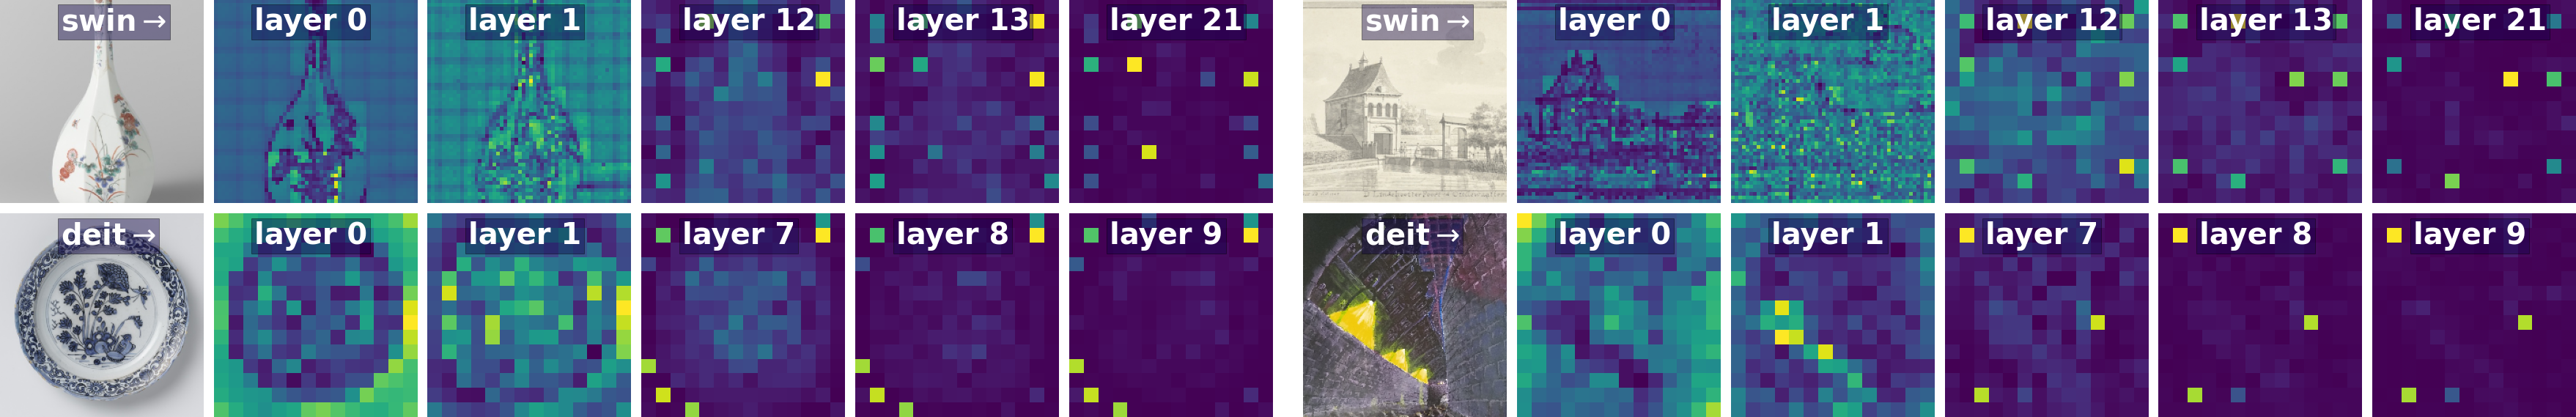
\includegraphics[width=\textwidth]{img/layers.png}

\centering
{\tiny \textbf{Saliency maps}}\\

\vspace{-0.3cm}
\begin{columns}
\column{0.5\textwidth}
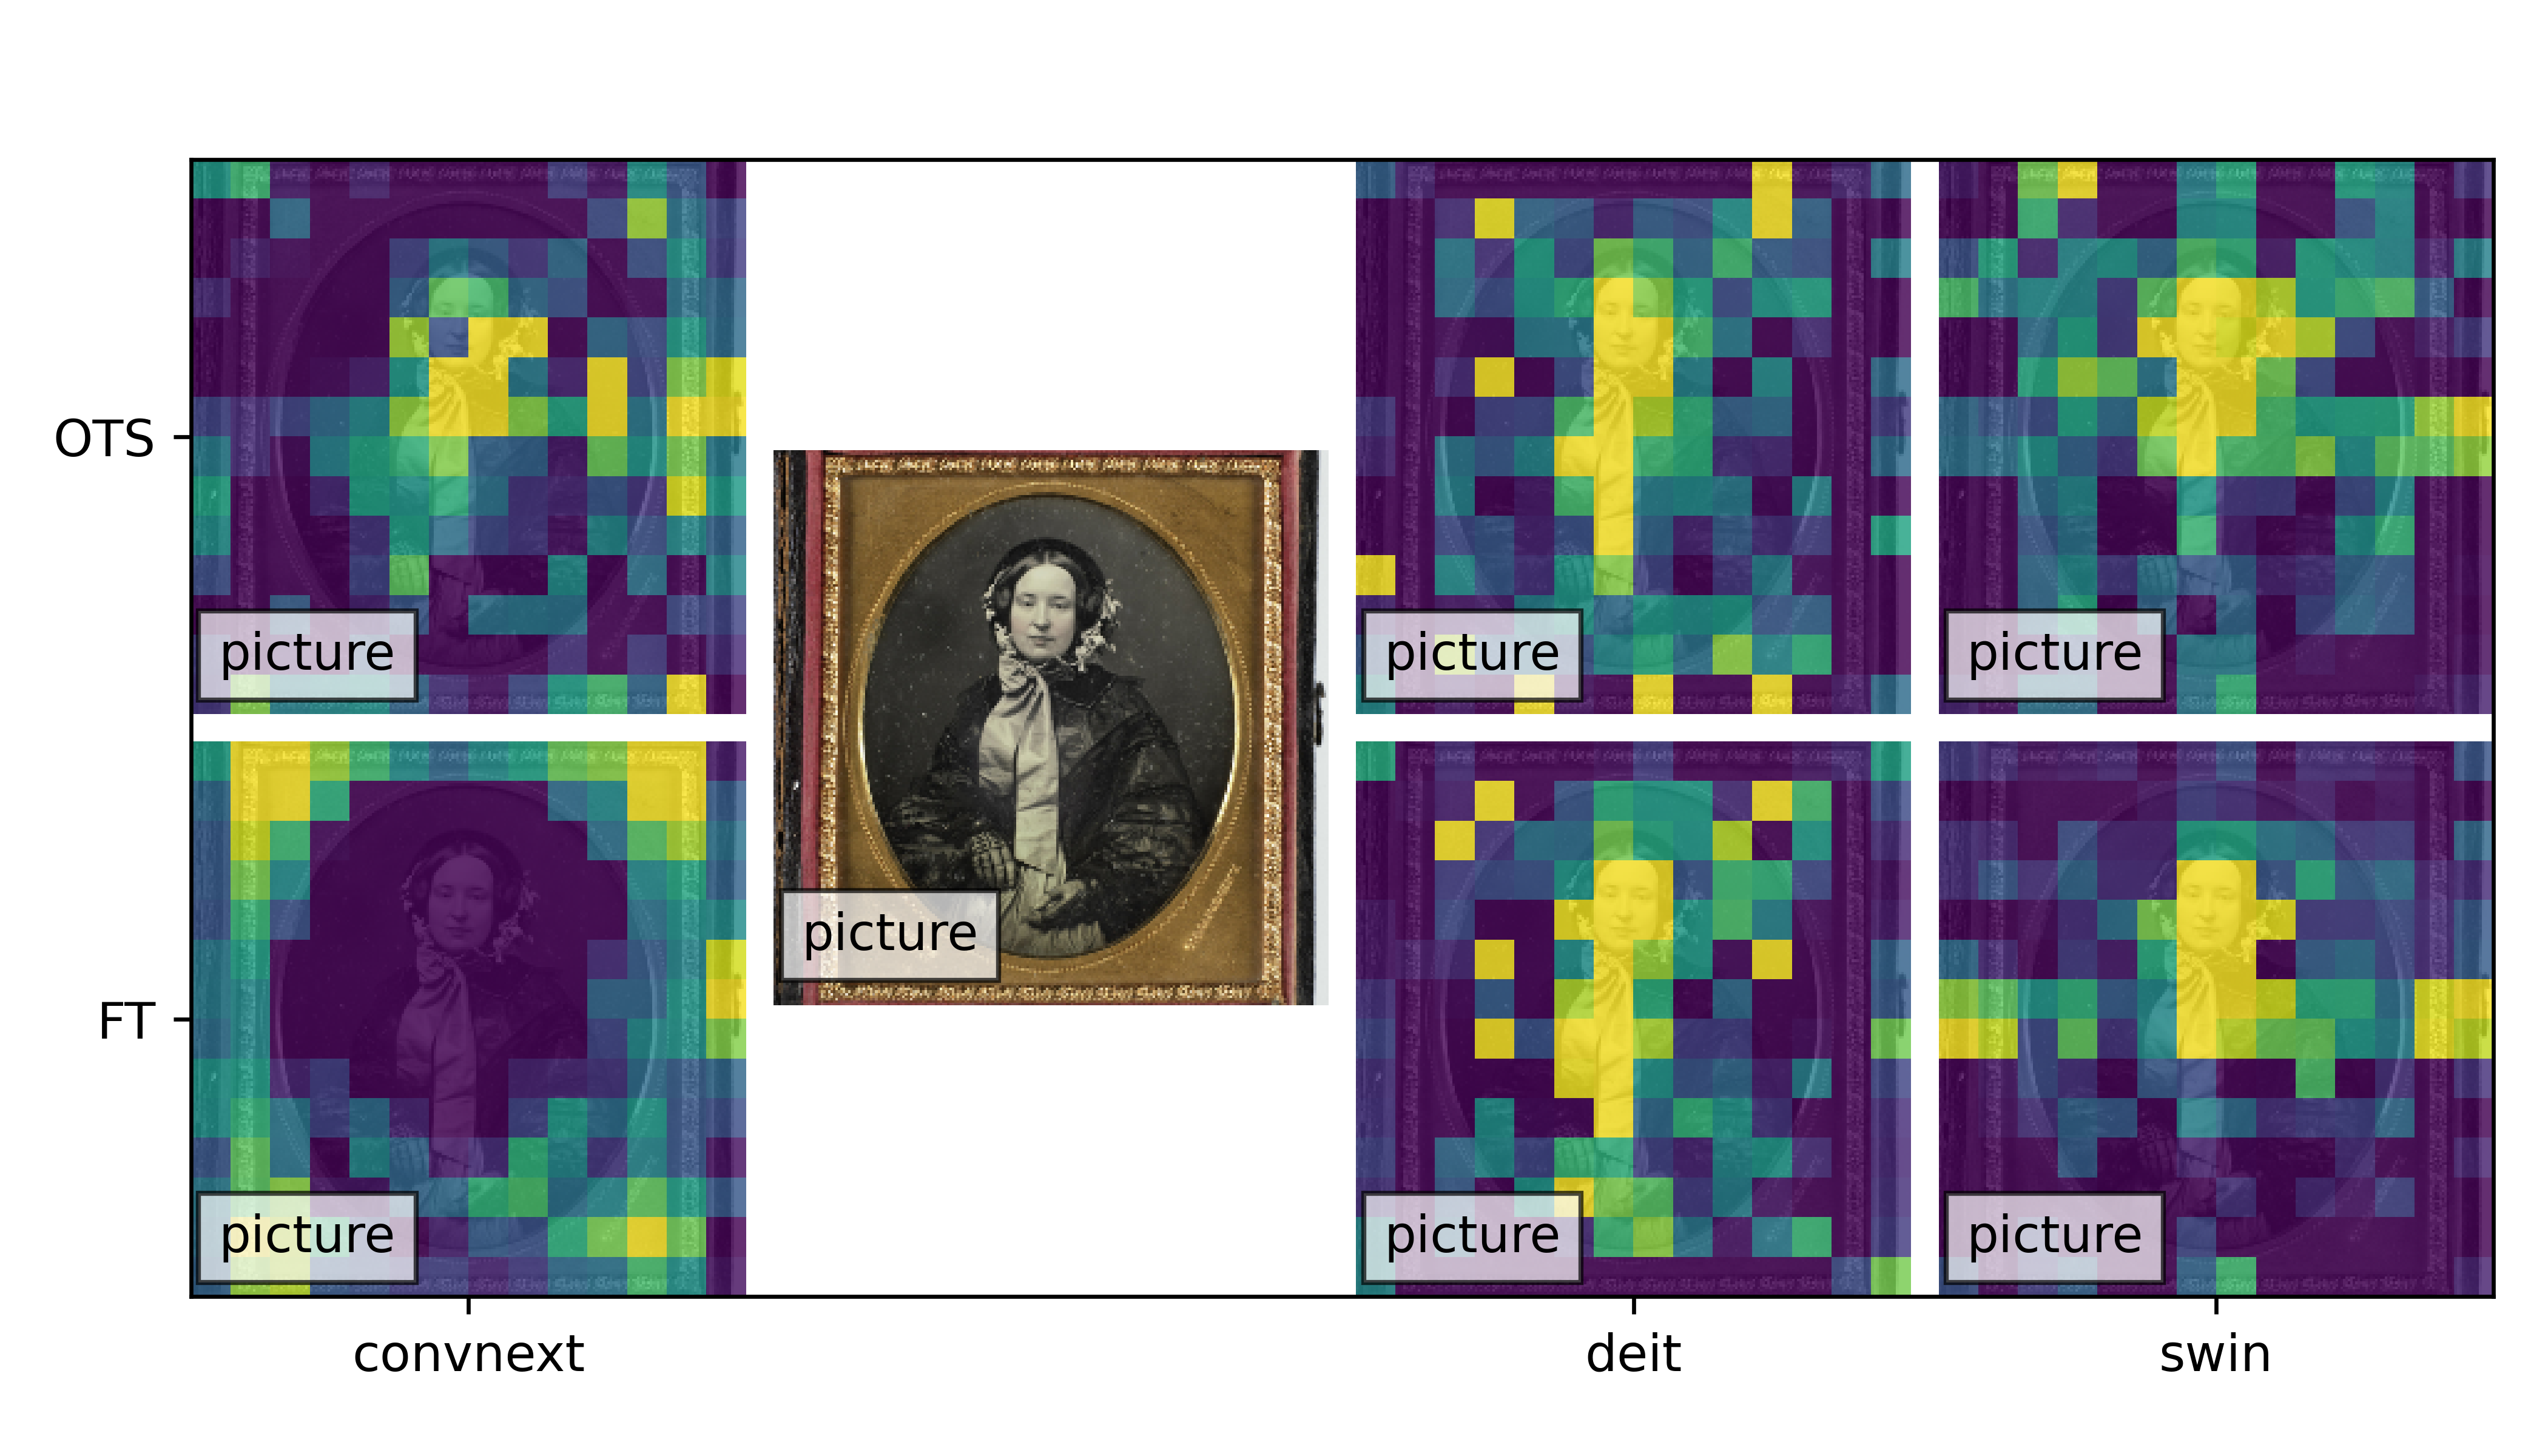
\includegraphics[width=\textwidth]{img/img011_salience.png}
\column{0.5\textwidth}
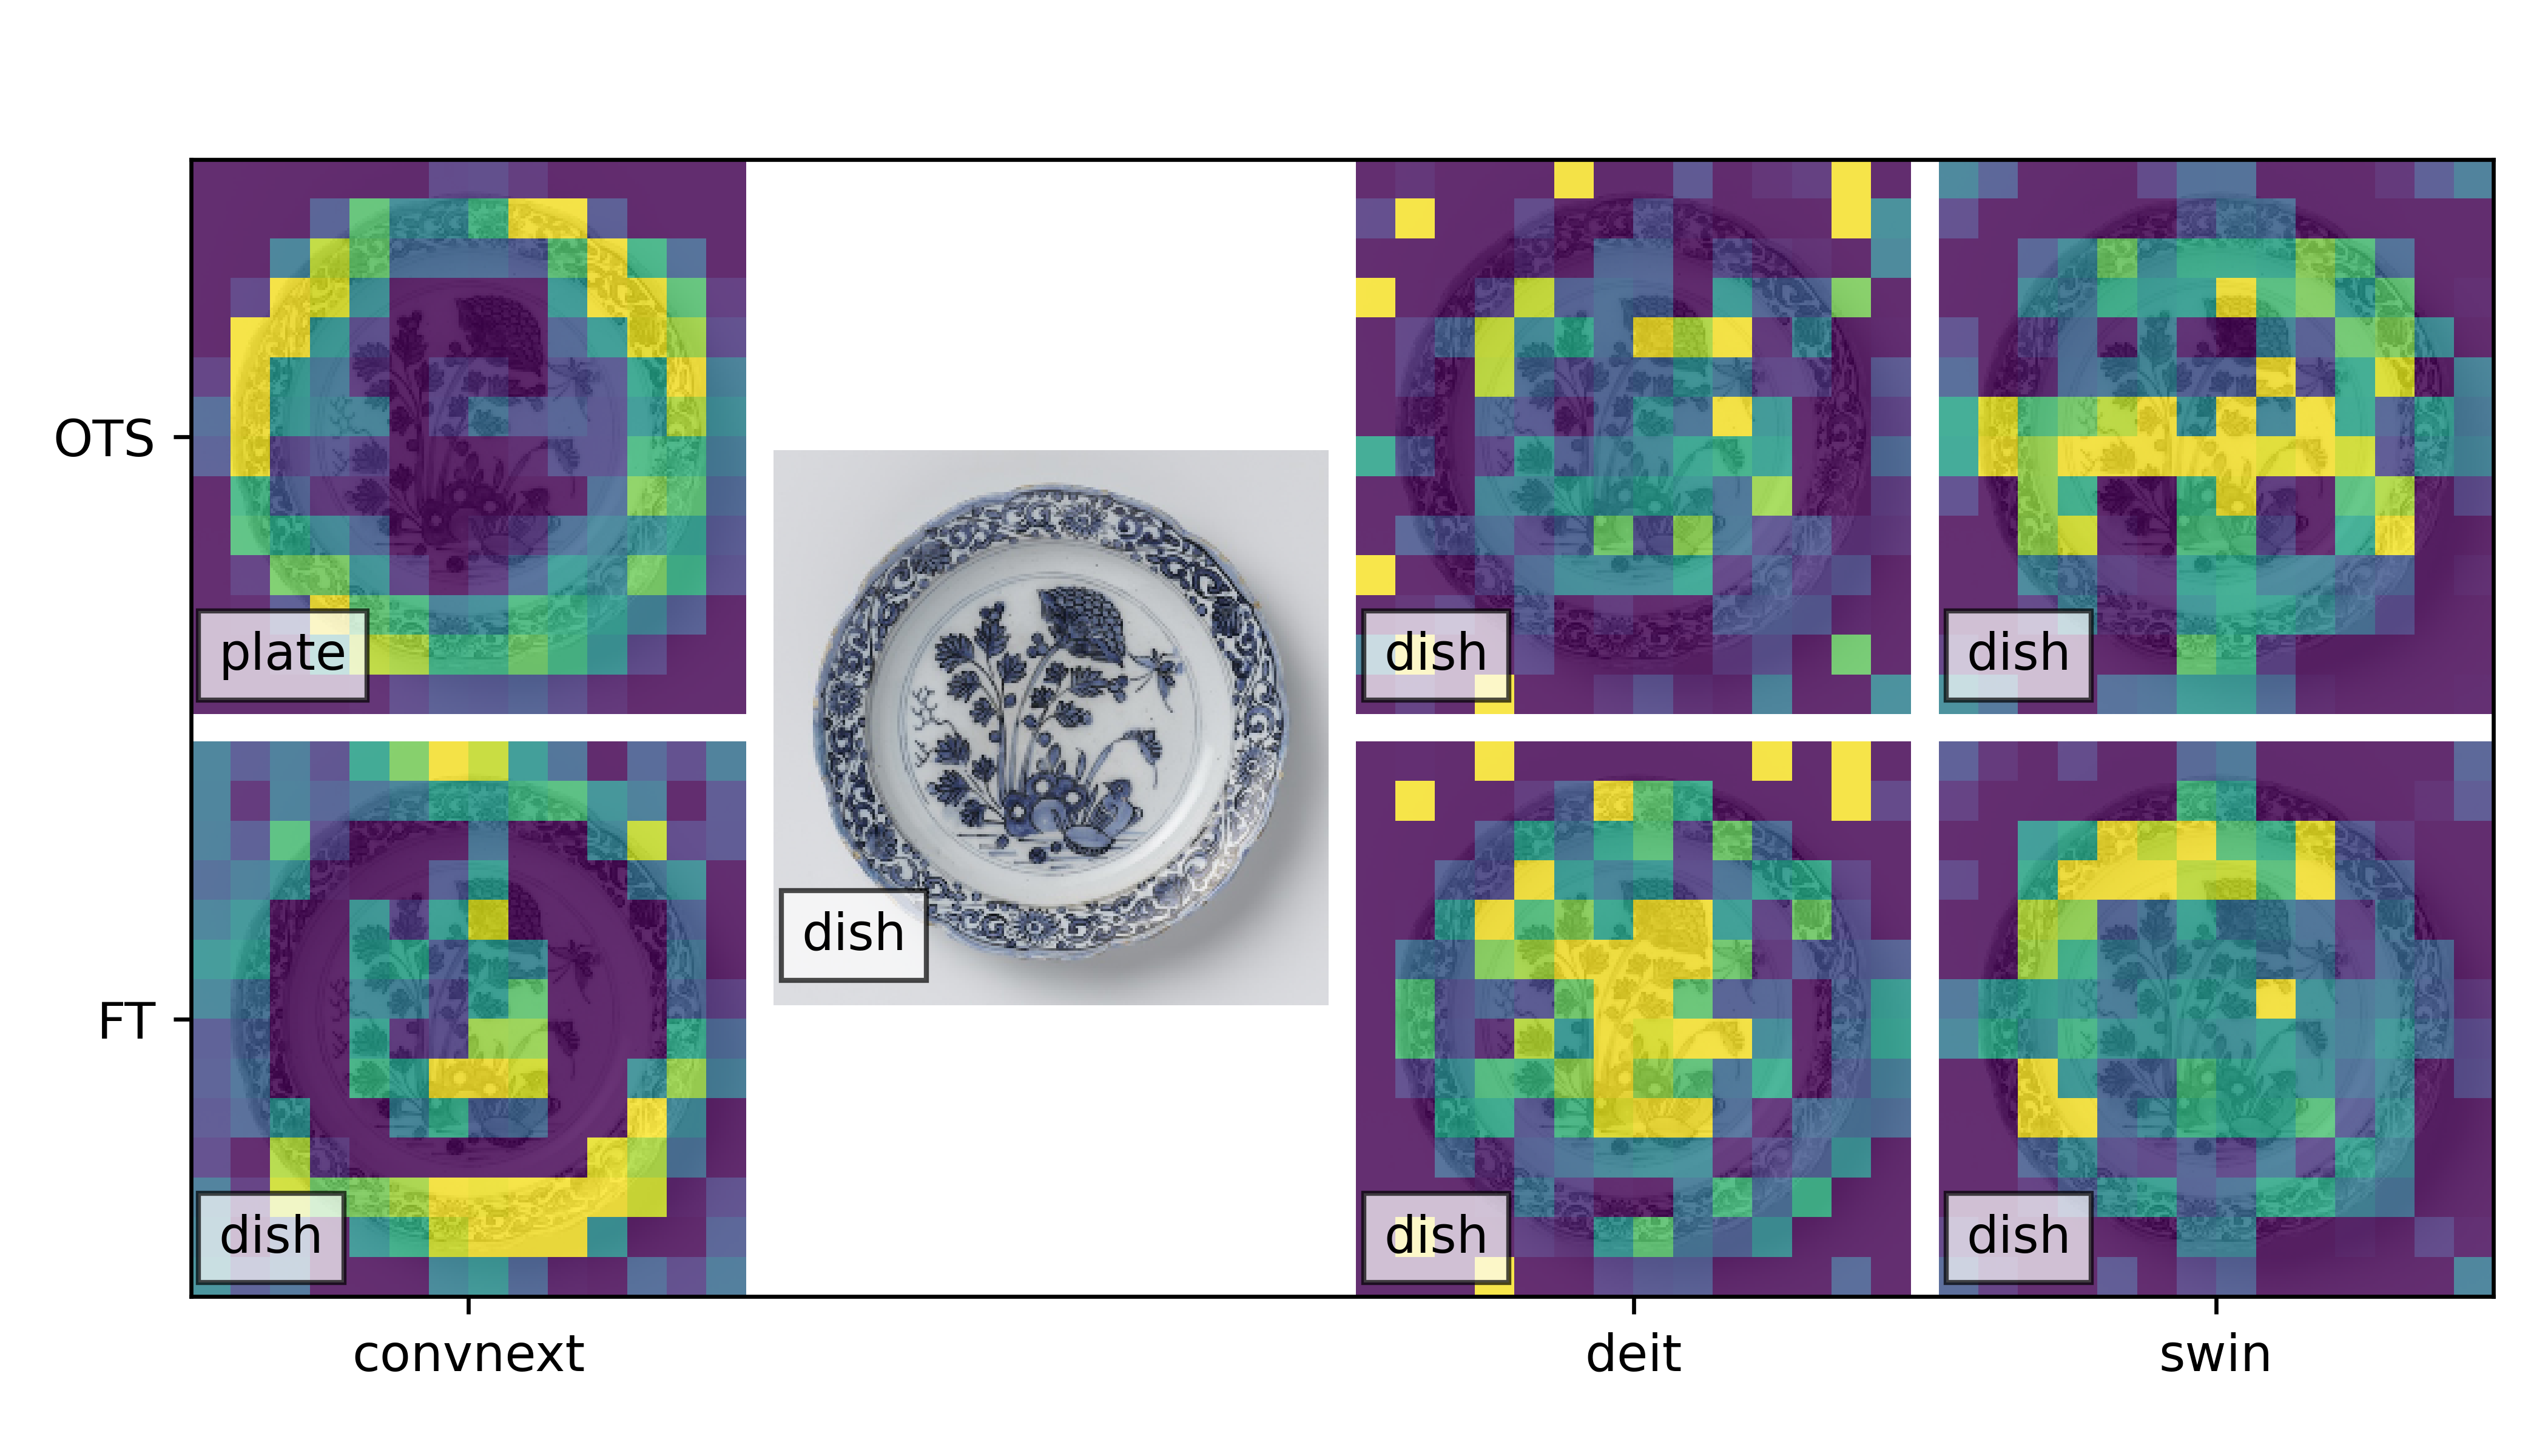
\includegraphics[width=\textwidth]{img/img005_salience.png}
\end{columns}
\end{frame}
%-------------------------------------------------------------------------------
